\documentclass[conference]{IEEEtran}
\IEEEoverridecommandlockouts
% The preceding line is only needed to identify funding in the first footnote. If that is unneeded, please comment it out.
\usepackage{cite}
\usepackage{amsmath,amssymb,amsfonts}
\usepackage{algorithmic}
\usepackage{graphicx}
\usepackage{textcomp}
\usepackage{xcolor}
\usepackage{amsmath,amssymb,amsthm}
\usepackage{graphicx}
\usepackage{caption}
\usepackage{subcaption,algorithm,calrsfs}
\def\BibTeX{{\rm B\kern-.05em{\sc i\kern-.025em b}\kern-.08em
    T\kern-.1667em\lower.7ex\hbox{E}\kern-.125emX}}
\begin{document}

\title{Cost Balancing Clustering with Unknown Values using Subspace Clustering
\thanks{Hyun was supported by NSERC CGS-M}
}

\author{\IEEEauthorblockN{Seung Gyu Hyun}
\IEEEauthorblockA{\textit{Cheriton school of computer science} \\
\textit{University of Waterloo}\\
Waterloo, Canada \\
sghyun@uwaterloo.ca}
\and
\IEEEauthorblockN{2\textsuperscript{nd} Given Name Surname}
\IEEEauthorblockA{\textit{dept. name of organization (of Aff.)} \\
\textit{name of organization (of Aff.)}\\
City, Country \\
email address or ORCID}
}

\maketitle

\begin{abstract}
Clustering is an important technique in machine learning and data mining
but traditional distance-based clustering algorithms may have difficulties when
values are missing in the dataset. We propose a cost-sensitive
subspace clustering model that determines which unknown features should be 
provided by the user in order to classify a point to its cluster. We then evaluate
this model using real-world datasets, and show that it performs comparably
to k-means but at a lower cost.
\end{abstract}

\begin{IEEEkeywords}
clustering, subspace clustering, machine learning
\end{IEEEkeywords}

\section{Introduction}
Clustering is one of the fundamental problems in machine learning with
many applications in the real world. Most clustering techniques measure the
`likeness' of two points through some distance or proximity metric. This requires
all values for every attribute to be known, but this is not always
possible as databases are often `dirty' or the value has not been provided by
the user yet. One way to combat this is to have a user input all missing
values, but this may be too costly or impossible (for example, confidential
information). On the other hand, using a machine learning model to impute
the unknown values may produce too many artifacts.

In this paper, we propose a hybrid approach; we will train a model 
with a complete dataset (no missing values) to learn
the boundary between the clusters. Then,
given a point with unknown values,  this model produces
a schedule of features that the user should provide considering the costs
associated with updating each value. In other words,
the model will guide the users about which features
they need to prioritize in order to most accurately find its cluster. This can be
used in prognosis to see how similar cases went with minimal costs, or
dynamically choose survey questions to find similar consumers.

Learning methods where wide-variety of costs are considered are
often referred to as cost-sensitive learning \cite{b6}\cite{b7}, while authors of
\cite{b8} define methods that consider specifically the cost of finding
feature values as test-cost sensitive learning. The main contribution of this 
paper is to extend such framework, which primarily deals with
classifications, to clustering. This is done through two steps:
\begin{itemize}
	\item Building a cost considering model which both forms the clusters
	and stores informations on the boundaries of the clusters.
	\item Using the above model to suggest order of feature updates and
	classify points into the preformed clusters.
\end{itemize}

\subsection{Approach and framework}
We begin by assuming the data (represented as feature vectors) is in a
metric space and that points that are similar in nature are also close in distance.
We further assume that any value of feature $f_i$ may be missing, but
can be provided by the user at cost $\mathfrak{C}(f_i)$. For any point
$p$, let $k(p)$ and $u(p)$ be the known and unknown features of $p$.
Finally, we will normalize all values to be between $[0,1]$, including 
$\mathfrak{C}(f)$.

In our setting, distance-based clustering becomes problematic. Most obviously,
it may be impossible to know \emph{which} centroid is closest to a feature
vector with missing values. For example, consider two centroids $c_1 = (1,0)$
and $c_2=(2,2)$ and a point with missing y-coordinate $p = (1,?)$; we cannot
say whether $p$ is closer to $c_1 $ or $c_2$. However, if we had a conditional
dependency of the distribution of the y-coordinate given $x=1$, then
the probability of which cluster $p$ belongs to is not uniform. Precisely, at
$p = (1,5/4)$, $p$ is equidistance to $c_1$ and $c_2$; thus
if $\Pr(y < 5/4 | x=1) > \Pr(y > 5/4 | x=1)$, then $p$ is more likely to be close
to $c_1$, and vice versa. This is the key idea of subspace clustering.

Subspace clustering algorithms attempt to cluster high dimensional data by 
projecting different partitions to different subspaces; this allows clustering
algorithms to search locally. These algorithms address the \emph{curse of
dimensionality} differently from feature selection: rather that judging which
features are redundant globally, they attempt to judge if certain features
are redundant \emph{conditioned} on being in some subspace \cite{b1}.

\section{Building the model}
In this section, we will describe our proposed tree-based unsupervised model:
the Cost Balancing Clustering Tree (CBCT). The basic outline follows the well-known
decision tree model \cite{b3}. Given a dataset $D$, we choose the
`best' feature and splitting value at each level greedily and recursively partition
$D$ until some stopping criteria. This can also be seen as an extension to the
CLusterTree model of \cite{b2} which further considers the cost of each split.

\subsection{Reward metric}
Given a set of data points $D$, define $c_D$ as its centroid and
$\delta_D$ as the average distance between the points in $D$ and $c_D$.
Define a \emph{boundary} to be a pair $(f,v)$, where $f$ is a feature and
$v$ is a value in the domain of that feature, and the left partition induced
by $b = (f,v)$ to be
$$ D_{(b,l)} = \{ p | p\in D, p[f] \le v \}. $$
Finally, the right parition induced by $b$ is $D_{(b,r)} = D \setminus D_{(b,l)}$.
We will quantify a boundary $b$ as a good split if the partitions induced by $b$
have lower average distance to their respective centroids compared to the
unpartitioned data.

\begin{figure}[H]
		\centering
		\begin{subfigure}[b]{0.3\linewidth}
			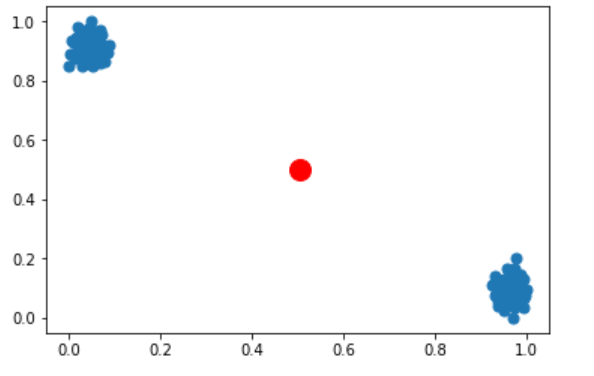
\includegraphics[width=\linewidth]{img01}
			\caption{no partition}
		\end{subfigure}
		\begin{subfigure}[b]{0.3\linewidth}
			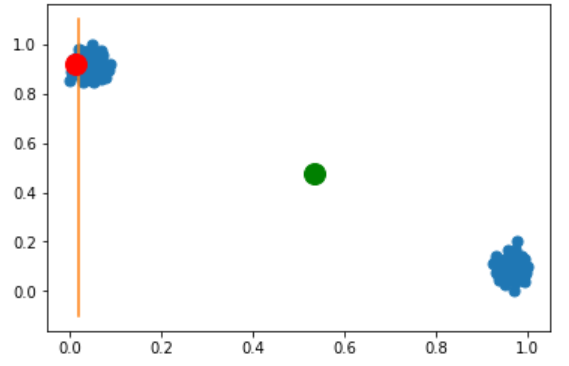
\includegraphics[width=\linewidth]{img02}
			\caption{$b_1=(x,0.02)$}
		\end{subfigure}
		\begin{subfigure}[b]{0.3\linewidth}
			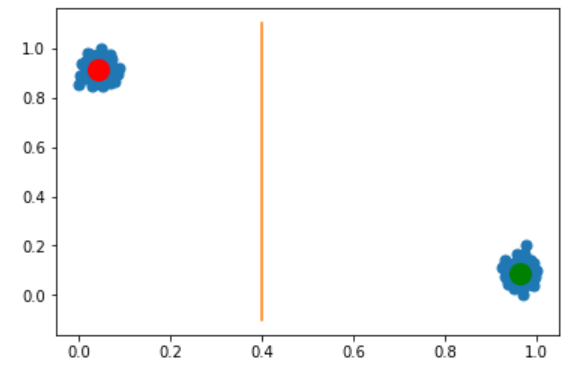
\includegraphics[width=\linewidth]{img03}
			\caption{$b_2=(x,0.4)$}
		\end{subfigure}
		\caption{Example of partitions induced by different boundaries}
		\label{fig1}
\end{figure}

Figure 1 shows a simple dataset with two example boundaries: 
$D_{(b_1,l)}$ has very few elements very close to $c_{(b_1,l)}$ but
$D_{(b_1,r)}$ has many elements very far from $c_{(b_1,r)}$; with $b_2$,
both partitions are close to their respective centroids. Intuitively, $b_2$ seems
to be a better split as the partitions that are induced are uniformly `tighter'.

Formally, we define the reward of splitting on a boundary $b$ as
\begin{align*}
	R(D,b) = p_l (\delta_D - \delta_{(b,l)}) + p_r (\delta_D - \delta_{(b,r)})
\end{align*}
where $p_* = |D_{(b,*)} | /  |D|$. Since $p_l + p_r = 1$, we can simplify the
above as $R(D,b) = \delta_D - (p_l \delta_{(b,l)} + p_r \delta_{(b,r)})$.

The reward function is essentially a weighted sum of the decrease in 
average distance to the centroids induced by a boundary $b$. The
term $\delta_D - \delta_*$ measures the decrease in distance while
$p_*$ is the ratio of the number of points in that partition. For 
$b = (f,v)$, the weigthed sum 
$p_l(\delta_D - \delta_{(b,l)}) + p_r (\delta_D -\delta_{(b,r)})$ can
also be viewed as the \emph{expected} decrease in distance from
knowing whether or not $p[f] > v$ as $p_l$ and $p_r$ are estimates of the
probability of being in each partition. Finally, we define the \emph{score}
of a split as the discounted reward:
$$ S(D,b) = R(D,b) - \alpha \mathfrak{C}(f) R(D,b) = 
    R(D,b) (1 - \alpha \mathfrak{C}(f)), $$
 where $\alpha \ge 0$ is a hyper-parameter and $\mathfrak{C}(f)$ is
 the cost of finding the value of feature $f$.
 
 \subsection{Algorithm for building CBCT}
 We finally outline a greedy algorithm to build a CBCT given training set
 $D$. At each node, we enumerate through the features and evenly spaced
 values from the domain of each feature in order to find a boundary 
 $b$ that maximizes the score $S(D,b)$. We stop when the number of data
 points are less than some threshold $\tau$ (although other stopping
 criteria are possible).
 
 In terms of complexity, at each node $n$, we examine $|D_n|$ elements
 $|\text{features}(D)| |\ell|$ times, where $|\ell|$ is the number of
 evenly spaced values. At any level, the total number of points in all nodes
 at that level cannot exceed $|D|$. For a tree of height $h$, this gives us the
 upper bound of $O(h |\text{features}(D)| |\ell| |D| )$. Also note that after
 using a feature $f$ in a split, we set $\mathfrak{C}(f) = 0$ for descendent
 nodes.

\begin{algorithm} 
   \textbf{build\_CBCT($D$)}\\
	Input: $D$ - dataset\\
	Output: $T$ - resulting tree 
	\begin{enumerate}
		\item if $|D| \le \tau$: return $T = (D,-,-)$
		\item for $f \in \text{features(D)}$:
		\begin{enumerate}
			\item $\ell = \text{linspace}(f_{min}, f_{max})$
			\item for $v \in \ell$:
			\begin{enumerate}
				\item $b_{(f,v)} := (f,v)$
				\item compute $S(D, b_{(f,v)})$
			\end{enumerate}
		\end{enumerate}
		\item $b_{max} = \text{arg max}_b S(D,b)$
		\item set $\mathfrak{C}(b_{max}.f) := 0$
		\item $T_{l} := \text{build\_CBCT}(D_{(b_{max}, l)})$
		\item $T_{r} := \text{build\_CBCT}(D_{(b_{max}, r)})$
	\end{enumerate}
\end{algorithm}

\section{Guiding the user}
Given a point $p$ with $u(p) \ne \phi$ (recall that $k(p)$ and $u(p)$ are
known and unknown features of $p$ resp.) and a preconstructed CBCT
$T$, this section will outline the various usages for $T$ to find different
information on $p$. 

\subsection{Suggesting next update}
From the unknown features, we want to suggest what feature to update
next such that if we were to stop updating the tuple after, we would have the
best approximation of the remaining unknown features as a function of
the known features. Since CBCT places the features that decreases the 
average distances to centroids (balanced with the cost) 
the most at the top, we can traverse
down $T$ using the known features and stop at the first unknown feature:
this is the feature that the model will suggest the user update next.

However, $p$ itself may not follow the hypothesis learned by $T$ and the
model should inform this to the user. In particular, traversing down $T$
is essentially finding the cluster that $p$ belongs to; the model has little
confidence of its suggestion if $p$ is dislike the found cluster. For some
node $n$, we can define a similarity score of $p$ to the points in that
node $D_n$ as
$$ \mathcal{S}(D_n,p) = \left(
\frac{1}{|D_n|} \sum_{p' \in D_n } \sqrt{ \sum_{f \in k(p)} (p'[f] - p[f])^2 } 
\right)^{-1}$$
which is the recipirocal of the average (L2) distance between $p$ and the points
of $D_n$, using only the known features. This value is higher when the
distance is smaller (i.e. $p$ is similar to points $D_n$). If the distance is zero
or there is no known feature, $\mathcal{S} = \infty$ since there is
nothing to contradict the model.

Next, let $\mathcal{N}_f$, for $f \in u(t)$, be the set of nodes that can be
reached by following these rules of traversal: at any node $n$, 1) if
the splitting feature is known, go down the appropriate branch; 2) if the
splitting feature is $f$, then go down both branches; 3) otherwise add
$n$ to $\mathcal{N}_f$. Intuitively, $\mathcal{N}_f$ is the set of all
nodes we could \emph{possibly} end at if $f$ was known and we traverse
$T$ until the first unknown feature. Finally, the confidence score of a particular
update suggestion is the expected similarity score:
$$ \mathcal{C}_1(T,p,f) = \sum_{n \in \mathcal{N}_f} \Pr(
\text{terminate at node n} | k(t) ) \mathcal{S}(D_n, p), $$
where we approximate the probability of terminating at a certain node as
$|D_n| / \sum_{i \in \mathcal{N}_f} |D_i|$. The lower this score, the less confident
the model is about the suggestion being the most beneficial.

\begin{algorithm}
\textbf{compute\_$\mathcal{N}_f(T, p)$} \\
Input: $T$ - tree; $p$ - point \\
Output: $\mathcal{N}_f$
\begin{enumerate}
	\item if $T$ is empty: return $\{ \}$
	\item if $T$ is a leaf: return $\{ T.\text{node} \}$
	\item set $b$ to be the boundary at current node
	\item if $p[b.f]$ is known:
	\begin{enumerate}
		\item if $p[b.f] > b.v$: 
		return compute\_$\mathcal{N}_f(T.\text{right}, p)$
		\item else: return compute\_$\mathcal{N}_f(T.\text{left}, p)$
	\end{enumerate}
	\item else if $b.f = f$:
	\begin{enumerate}
		\item $N_{f}^{(r)} = \text{compute\_}\mathcal{N}_A(T.\text{right},t)$
		\item $N_{f}^{(l)} = \text{compute\_}\mathcal{N}_A(T.\text{left},t)$
		\item return $N_{f}^{(r)} \cup N_{f}^{(l)}$
	\end{enumerate}
	\item else: return $\{ T.\text{node} \}$
\end{enumerate}
\end{algorithm}

\subsection{Classifying $p$'s cluster}
We will combine two metrics to classify which cluster $C_n$ the point
with uncertainty $p$ belongs to: the probability of any point belonging to
$C_n$ and the similarity between $k(t)$ and the points in $C_n$. The reason
behind this is simple; suppose $C_1$ has larger number of points (thus is
more frequent) than $C_2$ but the elements of $C_2$ are more similar to
$t$, then these two quantities must be balanced in order to effectively judge
with cluster $p$ belongs to.

Let $\mathcal{N}$ be the set of nodes reachable probabilistically by using all
unknown features (as opposed to $\mathcal{N}_f$ which only used feature
$f$). For each $n \in \mathcal{N}$, we give a confidence score that
$p$ belongs to $C_n$ as
$$ \mathcal{C}_2(T,p,n) = p_n \mathcal{S}(D_n, p) $$
where $p_n = |D_n|/\sum_{i\in \mathcal{N}} |D_i|$. We then present
to the user a list of possible clusters ordered by their $\mathcal{C}_2$ scores.
We also supply simple repair functions mean, median, and mode impoutations,
akin to \cite{b4}, which can be used for data cleaning (itself a large field with
vast industrial applications).

\begin{algorithm}
\textbf{compute\_$\mathcal{N}(T,p)$}\\
Input: $T$ - tree; t - tuple \\
Output: $\mathcal{N}$
\begin{enumerate}
	\item if $T$ is empty: return $\{ \}$
	\item if $T$ is a leaf: return $\{ T.\text{node} \}$
	\item let $b$ be the boundary at current node
	\item if $t[b.f]$ is known:
	\begin{enumerate}
		\item if $t[b.f] > b.v$: return compute\_$\mathcal{n}(T.\text{right},p)$
		\item else: return compute\_$\mathcal{n}(T.\text{left},p)$
	\end{enumerate}
	\item else:
	\begin{enumerate}
		\item $\mathcal{N}^{(r)} =$ compute\_$\mathcal{n}(T.\text{right},p)$
		\item $\mathcal{N}^{(l)} =$ compute\_$\mathcal{n}(T.\text{left},p)$
		\item return $\mathcal{N}^{(r)} \cup \mathcal{N}^{(l)}$
	\end{enumerate}
\end{enumerate}
\end{algorithm}

Finally, the difference in $\mathcal{C}_2$ scores before and after an update
may be used to catch erroneous updates. If $p$ follows the hypothesis
learned by the model, the top confidence score $\mathcal{C}_2$ will
increase as we receive more user-provided values. On the other hand,
if the model receives a value that was not expected, which makes the
hypothesis less likely to apply, then the confidence will decrease. Thus,
if an update leads to a large change in the top $\mathcal{C}_2$ score in
the negative direction (this is a loss of confidence), we should inform the user. 
Let $p'$ be a tuple with a single update from $p$, then report
$$ \mathfrak{C_3}(T,p,p') = \max_n \mathcal{C}_2 (T,p',n) -
	\max_n \mathcal{C}_2(T,p,n).$$

\section{Experimental results}
The algorithms above were implemented using C++ with the goal of
assessing the practical performance using real-life datasets \cite{b5}.
We divide roughly 90\% of the data as the training
set and the rest as the test set. We use the training set to build a CBCT and
simulate user interaction by dropping random subset of the features for each
tuple in the test set and provide those values as needed.

\subsection{Case study I}
For the first case study, we used the Heart Disease UCI . This dataset has
13 features related to test results and a label indicating the presence of heart
disease in patients.  To avoid overfitting, we also prune the tree such that
the height does not exceed 7, which was found to work well using 
cross-validation. 

First, we will compare the performance of CBCT with uniform costs to $k$-means.
For CBCT, we measure the distance from $p$ to the centroid of the
cluster with the highest $\mathcal{C}_2$ score. From $k$-means, we will use
the training set to $k=50$ centroids (again chosen through cross-validation)
then measure the minimal distance between $p$ and a centroid only
using $k(p)$. Figure \ref{fig2} shows that the average distance decrease
faster for the CBCT than $k$-means but the minimum distances achieved
in both clustering algorithm is comparable. The flattening of the curve
for the CBCT is due to the pruning.

Next, we compare the performances of a CBCT built with uniform costs to
one built with (normalized) costs provided from the Ontario Health 
Insurance Plan's
fee schedule. Certain tests are `grouped', meaning performing a test provides
values for multiple features. Figure \ref{fig2} shows that using uniform
cost and the actual cost performs similarly (decreasing faster than
$k$-menas), but the average cost is noticibly smaller with the actual cost
compared to the uniform cost, which itself is smaller compared to $k$-means.

\begin{figure}[H]
		\centering
		\begin{subfigure}[b]{0.4\linewidth}
			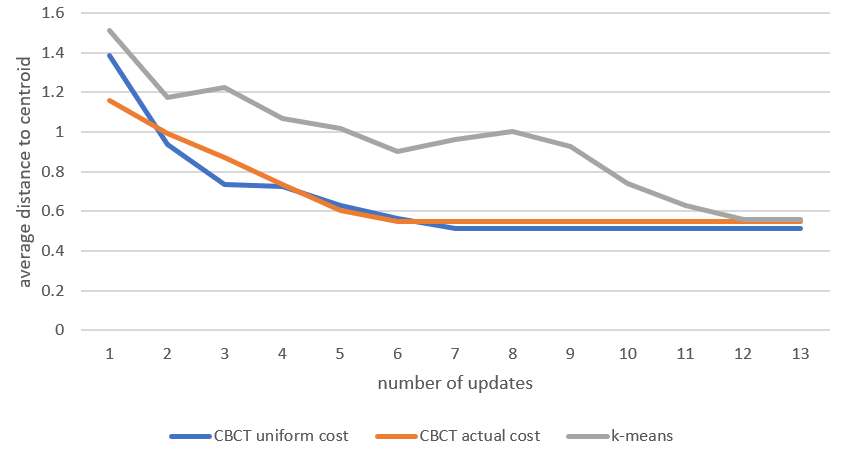
\includegraphics[width=\linewidth]{img05}
			\caption{average distances}
		\end{subfigure}
		\begin{subfigure}[b]{0.4\linewidth}
			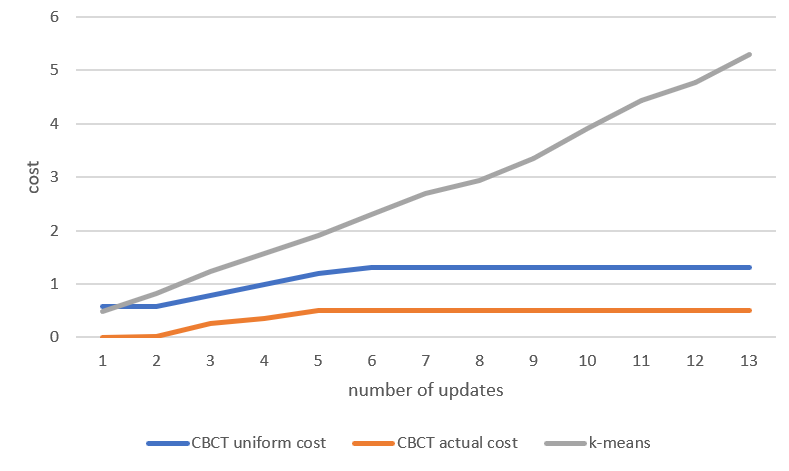
\includegraphics[width=\linewidth]{img06}
			\caption{average costs}
		\end{subfigure}
		\caption{CBCT uniform cost vs CBCT actual cost vs k-means}
		\label{fig2}
\end{figure}

\subsection{Case study II}
For this case study, we use the Wine Data Set, which has 13
features. In this dataset, the cost is not provided, so we will set each cost
to be the same value. Recall that the score of the split $S(D,b)$ is the discounted
reward and that after a feature $f$ is used, $\mathfrak{C}(f)$ is set to zero.
This means that at uniform cost, the value we set is essentially the
`willingness' to use an unused feature for the next split. In order to be
cost-efficient, we will set the cost to be high (at 0.8). 

Again, figure \ref{fig3} shows that using the updates suggested by a
CBCT decreases the average distances faster and more cost efficiently than
randomly choosing features. This is especially evident for the first update
in this dataset.
\begin{figure}[H]
		\centering
		\begin{subfigure}[b]{0.4\linewidth}
			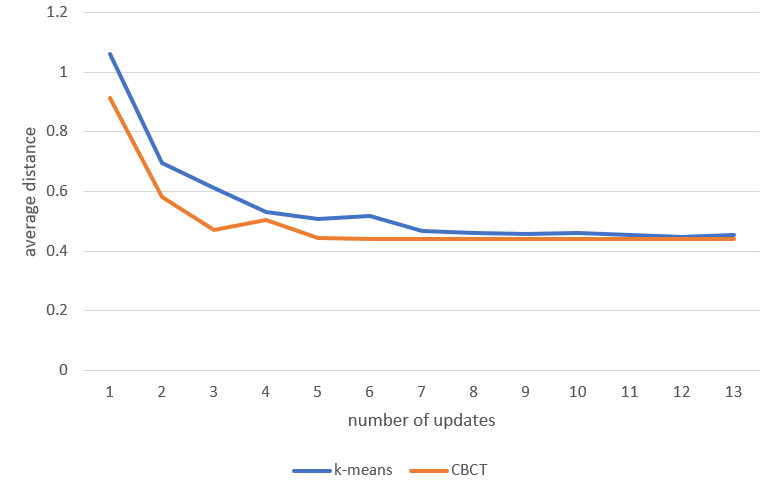
\includegraphics[width=\linewidth]{img08}
			\caption{average distances}
		\end{subfigure}
		\begin{subfigure}[b]{0.4\linewidth}
			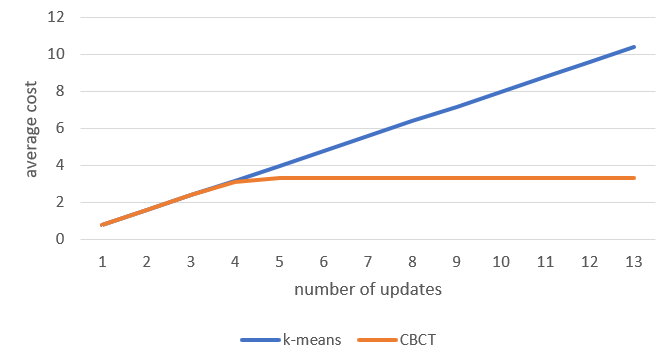
\includegraphics[width=\linewidth]{img09}
			\caption{average costs}
		\end{subfigure}
		\begin{subfigure}[b]{0.4\linewidth}
			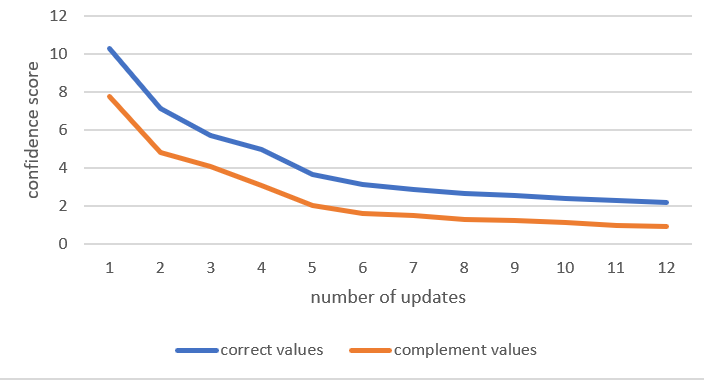
\includegraphics[width=\linewidth]{img10}
			\caption{average costs}
		\end{subfigure}
		\caption{CBCT uniform cost vs k-means}
		\label{fig3}
\end{figure}

Finally, figure
\ref{fig3} also by shows the confidence score of the update suggestions 
($\mathcal{C}_1$) when: 1) the correct values are given; 2) the complement
values are given. In the latter case, the points generated tend to be dissimilar
to other points, thus does not follow closely the hypothesis learned by the model.
In both cases, the confidence that an update will help drops as we supply
more values (as expected), but it decreases more slowly with the correct values.


\section{Discussion and Future Works}
When trying to classify a point $p$ to a cluster, the CBCT attempts to
improve two aspects: giving better update suggestions than randomly
choosing features, and finding and judging possible clusters that $p$ could
belong to. The experimental results of the previous section suggest that
the CBCT performs similarly to $k$-means with complete datasets, but
reaches the minimum distances faster and more cost efficiently. 

These improvements are best used in situations where there is a large
repository of complete historical data, yet obtain new data is expensive
such as in healthcare or education. This could be of particular interest in
education as the advent of online learning has allowed for more personalized
learning, but this requires fast identification of classes of learners, that is
identify the cluster which the learner belongs to. 

There are several avenues to investigate in the future. First, we can see how
different reward functions affect the choice of splits. For example,
rather than minimizing the distances induced by a boundary, we can
maximize the purity of the partition using the Gini impurity, which has already
been used in decision tree classifiers as an alternative to entropy.

There is also an alternative way to view this problem. If we view
the specific combination of $(k(p),u(p))$ as a state, then finding the next
feature update could be stated as a Markov Decision Process (MDP) problem.
This idea was used in \cite{b9} and \cite{b8} for classification, and it would
be interesting to find a parallel in clustering.


Finally, it is intersting to consider how human-in-the-loop feature updates
can interact with completely automatic repairs. The features at higher in
the CBCT are deemed to carry more importance; thus, knowing them should
theorectically also assist other algorithms. We could, for instance, see if
following the schedule of updates given by the CBCT improves the 
performance of a matrix completion algorithm compared to randomly supplying
values.


\begin{thebibliography}{00}
\bibitem{b1}  Lance Parsons, Ehtesham Haque, and Huan Liu. Subspace clustering for high dimensional
data: A review. SIGKDD Explor. Newsl., 6(1):90–105, June 2004.
\bibitem{b2} Bing Liu, Yiyuan Xia, and Philip S. Yu. Clustering through decision tree construction. In Proceedings of the Ninth International Conference on Information and Knowledge Management,
CIKM ’00, page 20–29, New York, NY, USA, 2000. Association for Computing Machinery.
\bibitem{b3}  J. R. Quinlan. Introduction of decision tree. Machine Learning, 1986
\bibitem{b4} Sanjay Krishnan, Michael J Franklin, Ken Goldberg, and Eugene Wu. Boostclean: Automated
error detection and repair for machine learning. arXiv preprint arXiv:1711.01299, 2017.
\bibitem{b5}C. L. Blake and C. J. Merz. UCI repository of machine learning databases, 1998
\bibitem{b6} C. Elkan. The foundations of cost-sensitive learning. In
Proc. of the IJCAI01, pages 973–978, 2001.
\bibitem{b7} ] P. D. Turney. Types of cost in inductive concept learning.
In Workshop on Cost-Sensitive Learning at the 17th International Conference on Machine Learning, 2000.
\bibitem{b8} Xiaoyong Chai, Lin Deng, Qiang Yang, and Charles X. Ling. 2004. Test-Cost Sensitive Naive Bayes Classification. In Proceedings of the Fourth IEEE International Conference on Data Mining (ICDM ’04). IEEE Computer Society, USA, 51–58.
\bibitem{b9} V. B. Zubek and T. G. Dietterich. Pruning improves heuristic
search for cost-sensitive learning. In Proc. of ICML02, pages
27–34, Sydney, Australia, 2002.
\end{thebibliography}

\end{document}
